\documentclass[12pt,a4paper,titlepage]{report}
\usepackage[utf8]{inputenc}
\usepackage[portuguese]{babel}
\usepackage[T1]{fontenc}
\usepackage{fancyhdr}
\usepackage{amsmath}
\usepackage{amsfonts}
\usepackage{amssymb}
\usepackage{makeidx}
\usepackage{graphicx}
\usepackage{lmodern}
\usepackage{wrapfig}
\usepackage{color}
\usepackage{float}
\usepackage{fourier}
\usepackage[left=2cm,right=2cm,top=1cm,bottom=2cm]{geometry}
\author{Bartolomeu J. Ubisse}
\pagestyle{fancy}
\renewcommand{\headrulewidth}{0pt}
\renewcommand{\footrulewidth}{1pt}
\fancyfoot[L]{\tt B.Ubisse \& H. Marrenjo | UEM - 2017}
\fancyfoot[c]{}
\fancyfoot[r]{\thepage}
\begin{document}


\begin{figure}[htb]

\centering

\includegraphics[scale=1]{UEM-logotipo}
\end{figure}
\centering
{ \Large Universidade Eduardo Mondlane}\\[0.3cm] 
\large Faculdade de Ci\^encias\\[0.2cm]
 \large Departamento de F\'isica\\[0.5cm]

\textsc{Electr\^onica B\'asica} \\[1cm]
\begin{flushleft}
\tt 2017-AP\# 4-Transistores de Efeito de Campo (FETs)\\
\hrulefill
\end{flushleft}

\begin{enumerate}
\item Explique o que entende por um transistor de efeito de campo (FET) e em que difere de um TBJ. 
\item Explique como \'e que pode avaliar o estado de um JFET de canal n, i.\'e, se est\'a ou n\~ao avariado.
\item Explique porque \'e que se diz que o FET \'e unipolar.
\item Quais s\~ao as aplica\c c\~oes de um JFET?
\item D\^e exemplos de um circu\'ito discreto e um integrado.
\item Determine as magnitudes dos resistores do circu\'ito da fig.\ref{a2} considerando que $V_p = -3$V, $I_{DSS}=9$mA, $V_G=5$V, $I_D=4$mA e $V_D=11$V. i)- Baseando-se em modelo de pequenos sinais, determine o ganho de tens\~ao ($A_v$).
  \begin{figure}[H]
\centering
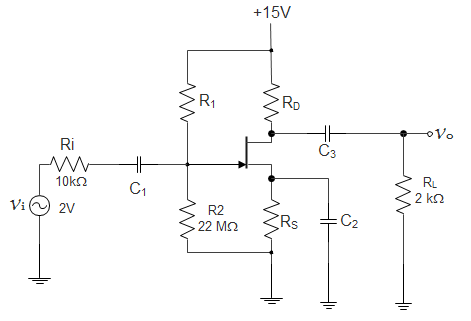
\includegraphics[scale=0.7]{JFET1}
\caption{}
\label{a2}
\end{figure}

\item Explique o que entende por tens\~ao de estrangulamento (\textit{pinch-off voltage}).
\item Explique o mecanismo de funcionamento de um MOSFET de canal n de tipo enriquecimento.
\item Explique porque raz\~ao a tecnologia MOS \'e a mais usada no fabrico de circu\'itos integrados em escala muita alta de integra\c c\~ao (VLS - very-large-scale integration).
\item Explique o que entende por tens\~ao limiar ($V_{th}$- \textit{threshold voltage}). Especifique as condi\c c\~oes para as diferentes regi\~oes de funcionamento de um NMOS de enriquecimento.
\item Qual \'e o papel do $SiO_2$ nos MOSFETs?
\item Explique a principal diferença entre MOSFET de  intensificação e de depleção no aspecto construtivo.
\item Determine $R_D$ e $R_S$ do circu\'ito da fig.\ref{a} sabendo que  $I_D=0.4$mA  ,$V_{th}=2$V, $W/L=40$ e $\mu_n cox =0.02mA/V^{2}$.
\begin{figure}[H]
\centering
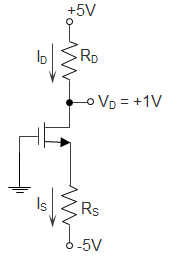
\includegraphics[scale=0.7]{MOSFET1}
\caption{}
\label{a}
\end{figure}

\item Determine as magnitudes dos res\'istores da fig.\ref{a1} de modo que a corrente de dreno seja de $1mA$ sabendo que, $V_{th}= 1V$, $K=1mA/V^2$ e a queda de tens\~ao em cada um dos resistor ($R_S$ e $R_D$) \'e $1/3$ da voltagem fornecida. i)- Determine as tens\~oes nodais.
 
\begin{figure}[H]
\centering
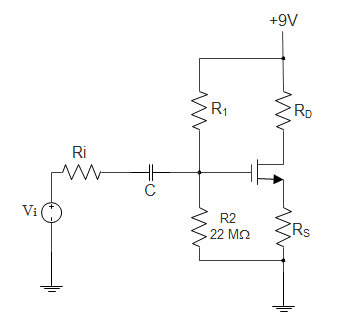
\includegraphics[scale=0.7]{MOSFET2}
\caption{}
\label{a1}
\end{figure}



\end{enumerate}







\end{document}